%!TEX root = main.tex
\section{Methods}\label{s:methods}


Traditional evolutionary algorithms (EAs) encode the biological process of evolution by natural selection in software so that they can be used to search for solutions to complex, high-dimensional problems~\cite{Eiben:2003tf}.  For example, the well-known genetic algorithm has been used to solve a wide-variety of engineering optimization problems~\cite{Goldberg:1989uj}, while genetic programming has consistently produced human-competitive results in fields as diverse as circuit layout and antenna design~\cite{Koza:2005wg,Lohn:2004to}.

{\em Markov Network Brains} (MNBs) are probabilistic automata that can be evolved via genetic algorithms~\cite{Edlund:2011kt}.  MNBs comprise a series of {\em gates}, where each gate accepts input and produces output, much like a neuron in an artificial neural network.  Each gate is itself governed by an evolved truth table.  
%
These truth tables may be binary, in which case the corresponding gate implements a small logic circuit, as shown in Table~\ref{t:logic-gate}.  Gates may also be probabilistic, in which case the evolved truth table contains probabilities, as shown in Table~\ref{t:prob-gate}.  In all cases, input to and output from evolved gates are binary.  Gates are subject to mutation, which may alter the fan-in or fan-out of the gate, or ``rewire''  the gate to connect an input or output to a different {\em state variable}, which provide input, output, or hidden states to the entire MNB, as shown in Figure~\ref{f:mnb-example}.

\begin{table}[h]
    \centering
    \caption{Example truth table for an evolved logic gate.  $X$ and $Y$ are binary inputs, $Z$ is a binary output.  This truth table implements the logic function $Z=X \lor \lnot Y$, which highlights the ability of evolution to use non-standard logic functions.}
    \begin{tabular}{ll|l}
    \hline
        {\bf X} & {\bf Y} & {\bf Z} \\\hline
        0 & 0 & 1\\
        0 & 1 & 0\\
        1 & 0 & 1\\
        1 & 1 & 1\\
        \hline
    \end{tabular}
    \label{t:logic-gate}
\end{table}

\begin{table}[h]
    \centering
    \caption{Example truth table for an evolved probabilistic gate.  $X$ and $Y$ are binary inputs, $Z$ is a binary output.  The output ($Z$) of this gate is given as a probability based on the combination of inputs $X$ and $Y$.  For example, $P(Z=1)$ given $X=1$ and $Y=1$ is 0.25.}
    \begin{tabular}{ll|ll}
    \hline
        {\bf X} & {\bf Y} & {\bf P(Z=0)} & P(Z=1) \\\hline
        0 & 0 & 0.0 & 1.0\\
        0 & 1 & 0.95 & 0.05\\
        1 & 0 & 0.5 & 0.5\\
        1 & 1 & 0.25 & 0.75\\
        \hline
    \end{tabular}
    \label{t:prob-gate}
\end{table}

\begin{figure}
\centering
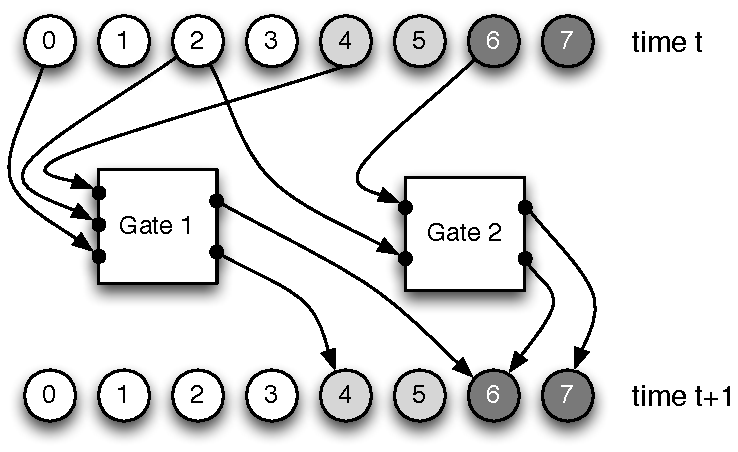
\includegraphics[width=0.45\textwidth]{markov-network-example}
\caption{An example Markov Network Brain (MNB) with 12 state variables: Four input states (white circles, 0-3), two hidden states (light grey circles, 4 and 5), two output states (dark grey circles, 6 and 7), and two gates (white squares, ``Gate 1" and ``Gate 2"). The MNB receives input in states 0-3 at time $t$, then each gate is activated, and their respective outputs are written into states 4, 6, and 7 at time $t+1$.}
\label{f:mnb-example}
\end{figure}

Figure~\ref{f:mnb-genome} depicts the {\em genome} for a MNB.  This genome is typically a circular list of integers ({\em codons}) that contains a series of {\em genes}.  Each gene encodes a single gate, and defines that gate's fan-in, fan-out, truth table, and the mapping of inputs and outputs to state variables.  The beginning of a gene is indicated by a {\em start codon}, a specified sequence of two integers, and the extent is determined by the size of the corresponding gate's truth table.  The entire genome is subject to mutation, including point-mutations (i.e., replacing a codon with a random integer), insertions (i.e., inserting a random sequence into the genome),  and deletions (i.e., deleting a random sequence from the genome).

\begin{figure}
\centering
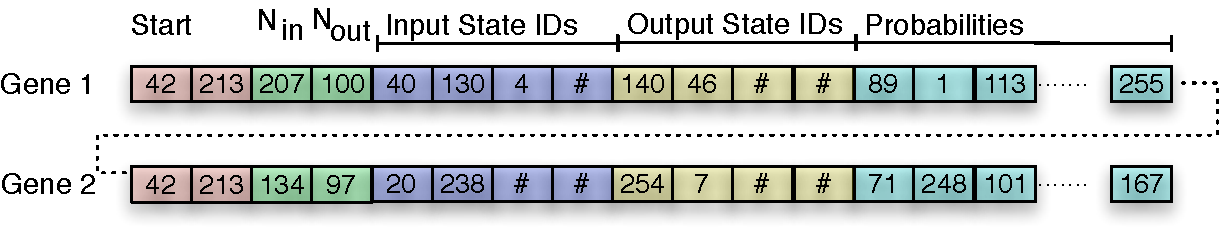
\includegraphics[width=.45\textwidth]{markov-network-genome}
\caption{Example genome containing two genes. The sequence (42, 213) is the start codon, and represents the beginning of a gate(red blocks). The next two codons describe the fan-in and fan-out of the gate (green blocks), and the following eight codons map inputs (blue blocks) and outputs (yellow blocks) to state variables.  The remaining codons comprise the gate's truth table (cyan blocks).}
\label{f:mnb-genome}
\end{figure}

While MNBs have most frequently been used to evolve controllers for agents in embedded environments~\cite{Edlund:2011kt,Olson:2013kx,Olson:2013ko}, we have recently begun applying MNBs to problems in engineering, specifically optical character recognition~\cite{Chapman:2013kf} and time-series forecasting (manuscript in preparation).  
%
MNBs have shown a remarkable ability to model state transitions that underlie a noisy physical process, as shown in Figure~\ref{f:mnb-model}.  Here, we will evolve MNBs to examine time-series data for abnormalities that are indicative of cancer.

\begin{figure*}
\centering
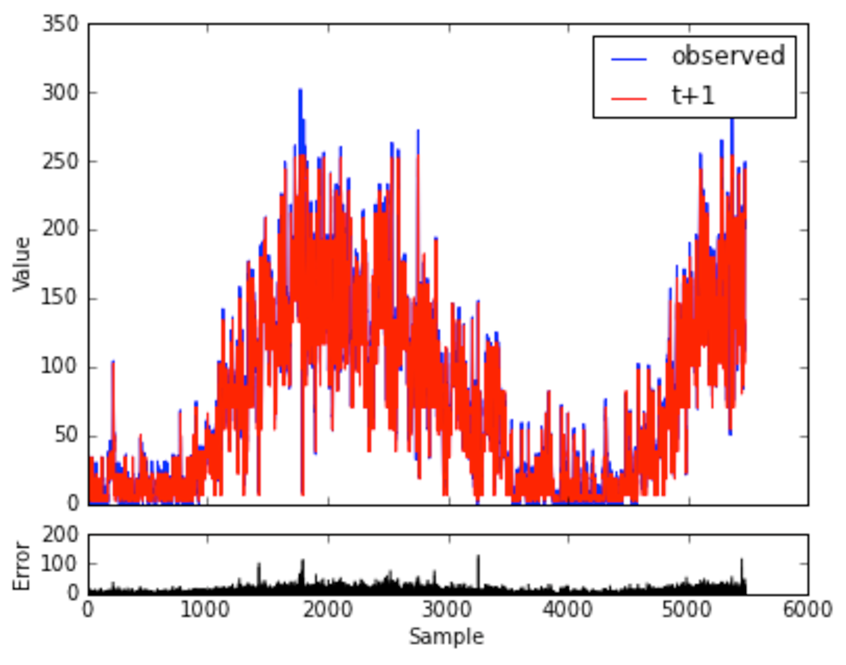
\includegraphics[width=.45\textwidth]{markov-network-sunspot}

\includegraphics[width=\textwidth]{markov-network-graph}
\caption{These figures show preliminary results of using MNBs to forecast space weather, specifically the daily number of sunspots visible from Earth.  This data is highly chaotic, and has a prediction horizon of 8 days.  At top we see a comparison of daily predicted vs.~observed sunspot numbers for the time period 1975 to 1989; at bottom is a depiction of the MNB that evolved to predict this time series.  These results indicate that MNBs are highly effective at time-series analysis.}
\label{f:mnb-model}
\end{figure*}





%This section describes the neuroevolutionary approach and the specific problem we addressed in this study.

% cellular automata
% traditional rule encoding, vis a vis game of life
% FSM rules
% PSM rules
% PSM adaptation
% evolutionary algorithm & FSMs/PSMs
% -- all parameters found online?

%
%\begin{figure}
%\centering
%\subfigure[]{\label{f:complex-frame0}\includegraphics[width=\HalfPage]{frame0001}}
%\hspace{1em}
%\subfigure[]{\label{f:complex-frame1}\includegraphics[width=\HalfPage]{frame0164}}
%\caption{Starting configuration of agents~\subref{f:complex-frame0} and position of agents 4s into a simulation~\subref{f:complex-frame1}.  White lines represent connections between agents; agents can transmit data only to those other agents to which they are connected.  The grid agents are to cover is outlined with black lines; $x$, $y$, and $z$ axis represented by red, green, and blue lines, respectively.}
%\label{f:grid-coveragea}
%\end{figure}
%
%\begin{table}[h]
%\centering
%\caption{Sensors and effectors of individual agents for the grid-coverage problem.}
%\label{t:agent}
%\begin{tabular}{ll p{11em}}
%\hline\hline
%Name & Type & Description\\\hline
%\code{rx0}\ldots\code{rx3} & sensor & directional radio receiver; each sensor covers a 90$^\circ$ ``pie slice'' around the agent\\
%\code{v0}\ldots\code{v2} & sensor & velocity vector $(x,y,z)$\\
%\code{p0}\ldots\code{p2} & sensor & absolute position $(x,y,z)$\\
%\code{f0}\ldots\code{f2} & effector & force vector $(x,y,z)$\\
%\code{tx} & effector & broadcasts a message to all agents within range; appropriate \code{rx} sensor is always set to the inverse of the distance between sender and receiver\\\hline
%\end{tabular}
%\end{table}

%\begin{table}[htb]
%\centering
%\caption{Relevant configuration parameters for {\neat}; those not listed are set to their default value.}
%\label{t:neat}
%\begin{tabular}{l l}
%\hline\hline
%Parameter & Value\\\hline
%PopulationSize & 100\\
%MaxGenerations & 200\\
%MutateAddNodeProbability & 0.03\\
%MutateAddLinkProbability & 0.05\\
%MutateDemolishLinkProbability & 0.03\\
%MutateLinkWeightsProbability & 0.8\\
%MutateOnlyProbability & 0.25\\
%MutateLinkProbability & 0.1\\
%AllowAddNodeToRecurrentConnection & 1.0\\
%AllowRecurrentConnections & 0.0\\
%AllowSelfRecurrentConnections & 0.0\\
%OnlySigmoidHiddenNodes & 1.0\\\hline
%\end{tabular}
%\end{table}
%
%
%
